
%%%%%%%%%%%%%%%%%%%%%%% file StudyWise_Chapter.tex %%%%%%%%%%%%%%%%%%%%%%%%%
%
% This is a chapter for Big Data in Education, edited by Al Essa and Dr. Kinshuk, Fall 2017
%
%%%%%%%%%%%%%%%%%%%%%%%%%%%%%%%%%%%%%%%%%%%%%%%%%%%%%%%%%%%%%%%%%%%

\documentclass[runningheads,a4paper]{llncs}

\usepackage{amssymb}
\setcounter{tocdepth}{3}
\usepackage{graphicx}
\usepackage{enumitem}
\usepackage{listings}
\usepackage{url}
\usepackage[T1]{fontenc}
\urldef{\mailsa}\path|{mark.riedesel, patrick.charles}@mheducation.com|
\newcommand{\keywords}[1]{\par\addvspace\baselineskip
\noindent\keywordname\enspace\ignorespaces#1}

\begin{document}

\mainmatter  % start of an individual contribution

% first the title is needed
\title{Learning Any Time, Anywhere:  Big Educational Data from Smart Devices}

% a short form should be given in case it is too long for the running head
\titlerunning{Spaced Practice Any Time, Anywhere}

% the name(s) of the author(s) follow(s) next
%
%
\author{Mark A. Riedesel
\and Parick Charles}
%
\authorrunning{M. A. Riedesel and P. Charles}
% (feature abused for this document to repeat the title also on left hand pages)

% the affiliations are given next; don't give your e-mail address
% unless you accept that it will be published
\institute{McGraw-Hill Education, 281 Summer Street, Boston, MA 02210
\mailsa}

%
% NB: a more complex sample for affiliations and the mapping to the
% corresponding authors can be found in the file "llncs.dem"
% (search for the string "\mainmatter" where a contribution starts).
% "llncs.dem" accompanies the document class "llncs.cls".
%

\maketitle


\begin{abstract}
For many people, especially young people, a smart phone is a constant companion.  Mobile apps which allow individuals to use a smart device to enhance their learning have the potential to be very useful for mastering basic educational material.  In order to evaluate and enhance the effectiveness of such applications when deployed at large scale, an infrastructure designed specifically for the collection of educational analytics data from such mobile apps is required.  

We detail here a set of applications and their associated infrastructure which was developed to allow students in courses using digital textbooks to enhance their knowledge of the basic course content anywhere and anytime by using their smart device to do spaced practice of the knowledge components of a course.  The power of current smart devices allows the entire application, including content and adaptive algorithm to be hosted and run locally on the user's smart device, so it functions fully even when no network connection is available.

The infrastructure for the collection and analysis of the educational analytics data is entirely cloud-based, using AWS S3 for data collection and storage, and the Apache Spark parallel computing framework for data analysis.  Thus, the entire system requires only laptop computers for the mobile developers who create the applications and this is also sufficient for the learning scientists who analyze the data.  Both the data collection system and the data analysis system can scale to handle the data from many millions of users with no modification to their architecture.  Similar architectures are now used for the Internet of Things (IOT) but have not yet been widely used for educational applications.

These applications have currently been deployed to thousands of users' smart devices and analytics data is being received from these users' smart devices from a wide range of locations on several continents.  In our highly connected world, this type of application will become much more common.  We describe here the type of infrastructure, security, and analytic methods needed to use these apps to advance learning and learning science.

\keywords{Spaced Practice,  Adaptive Flashcards, Mobile Learning, messaging systems, parallel computing, cloud computing}
\end{abstract}


\section{Introduction}

For many subjects, memorizing basic facts is an important first step in learning and mastering content.  In learning a foreign language, for example, basic vocabulary must be memorized as an essential part of learning syntax and grammar.  In medicine it is still considered essential for doctors, nurses, medical assistants, and EMTs to have basic knowledge of anatomy and physiology, pharmacology, and medical terminology memorized for immediate recall in critical situations.  Even for subjects which involve higher levels of cognition, retention of basic knowledge is commonly the foundation upon which higher levels of abstraction are built \cite{blume1956}.

Applications designed for long-term memorization are often conceptually based on models for human memory which grew out of early work on how memories decay with time but can be reinforced by repetition spaced in time \cite{ebbinghaus}.  Further research, particularly in the past twenty years, has shown that three related methods can help optimize the memorization of material:  spaced practice \cite{cepeda2008}, active retrieval  \cite{roediger2006,karpicke2008}, and interleaving \cite{stick2014}.

Spaced practice is a method where material one wants to learn is repeated on a schedule designed to reinforce decaying memories.  Ideally, an item (an atomic piece of knowledge) would be repeated just before it would otherwise be forgotten.  Using very specific models for the forgetting process allows mathematical optimization methods to be employed to produce optimal schedules for spaced practice\cite{pa2005,pa2008,mozer2016,settles2016}.

Active retrieval is the principle that requiring a learner to recall material in response to a challenge is more effective than re-reading material.   This is true even when there is some active involvement when reading, such as highlighting the most important parts of a passage.  So requiring a learner to respond to a question is significantly more effective than having the learner re-read a text containing the same basic piece of knowledge.  Questions can be in several modes such as multiple-choice single-answer, multiple-choice multi-answer, fill-in-the-blank, or matching.

Interleaving is a method where questions on different topics or sub-topics are intermixed.  It has been shown in learning arithmetic problems, for example, that mixing up different types of problems in practice sessions is more effective than concentrated drill on just one type \cite{rohrer2007}.

A learning program which can easily incorporate all three of these methods is through the use of flashcards.  Flashcards always require active retrieval and can also be timed and sequenced to incorporate spaced practice and inverleaving.  Manual methods of doing this have been used at least since the 1970's \cite{Leitner1972} but to implement a system which can optimize the user experience, a computer program is an especially effective way to accomplish this.  In a computer-based flashcard system, algorithms can be employed to create schedules for spaced practice which incorporate the user's record of correct and incorrect responses, the subject matter of each question, and the timing of the appearance of each item.

Several such systems have been deployed over the past twenty-five years or so.  These are typically designed for learning hundreds or thousands of facts over times extending over weeks, months, or years.  Such applications include SuperMemo, Anki, Duolingo, Brainscape, FireCracker, and Memorang [\url{http://www.supermemo.com}, \url{http://ankisrs.net}, \url{http://www.duolingo.com}, \url{http://www.brainscape.com}, \url{http://www.firecracker.me}, \url{http://www.memorangapp.com}].  Most of these applications require a web browser with an active network connection.  Those which have self-contained mobile versions which can operate off-line do not allow a centralized collection of user interaction data.  More academically based applications which do allow this have not yet been widely deployed \cite{Kam2009,Pavlik2016}.

With the smart devices currently available it is possible to develop self-contained mobile applications which include all of the educational content and which have the software needed to adaptively schedule spaced practice completely independent of a central computational service.  Such applications can generate user interaction data messages which can be sent to a central collection point.  Such data is needed for learning scientists to evaluate student performance and to further refine scheduling algorithms.  This allows users to make optimal use of their time in learning the material with these applications.  As large data sets accumulate, such data will also be very valuable for advancing basic understanding of the learning process.


\section{Mobile Practice of Course Content}

The Higher Education division of McGraw-Hill Education  (MHE) was interested in a way for students in a course using one of MHE's on-line, interactive textbooks, called SmartBooks [\url{http://www.mheducation.com/highered/platforms/smartbook.html}], to be able to use their smart phones to memorize some of the declarative knowledge presented in a title.  They quickly realized that a mobile phone application which had been developed to allow candidates in India to study for the U.S. Medical Licensing Exam (USMLE), called StudyWise, could be adapted for this purpose. 

This application was developed to utilize the existing homework questions from medically related titles and present them as flashcards on a smart mobile device.  The application was entirely self-contained, with the content, the user interface, and the scheduling algorithm all entirely contained on the smart device.  This allowed the application to function even when a network connection was not available, a requirement for use in areas with spotty  WiFi or cellular coverage.

It was recognized that this software could be re-targeted to provide optimized practice of course material within the time frame of a college semester by modifying the scheduling algorithm to optimize for practice of dozens to hundreds of items over a few weeks or months rather than the USMLE application which was designed for study of thousands of items over the course of one to two years.   By leveraging published research on learning and memory, a new algorithm was successfully developed which fit this use case \cite{Riedesel2017}.

\subsection{ Smart Device Mobile Applications}

As currently deployed, each of eight separate content titles has its own IOS and Android app.  Each app presents the homework questions in a title as an electronic flashcard, grouped by topic.  The questions, known as probes or items, come from MHE's existing Smartbook database of probes.  There are currently about 1500 SmartBook titles on a wide range of subjects.  For all of these titles combined there are some 2,350,000 distinct probes with almost three billion recorded answers for them from the web-browser-based SmartBook system.  

In SmartBook, each probe is associated with a knowledge component called a Learning Objective (LO).  The LOs are organized by topic, which in turn are related to the title's subject.  In a course that uses a SmartBook title, the instructor creates an assignment for a specified set of LOs.  Students see only probes associated with the LOs for that assignment, which they do on-line through a web browser.

StudyWise was designed as a mobile application which would allow students to practice all of the LOs in a title, organized by topic.  The mobile nature of the applications allows users to learn and master material whenever they have a few spare moments and wherever they happen to be.  The algorithm is designed to allow the learner to master each LO by repeated practice.  Once an LO's associated probes have been answered correctly three times, it is considered learned.

The fact that it is entirely self-contained on the mobile device means that it can be used whenever the user has a few spare minutes.  The pattern of session durations suggests shows that these applications are indeed being used primarily for a few minutes at a time, as can be seen in Figure \ref{fig:SessionDurationHistogram}.  This is rather different from the originally envisioned usage model, which was for dedicated 30 minute sessions each day.

\begin{figure}
\centering
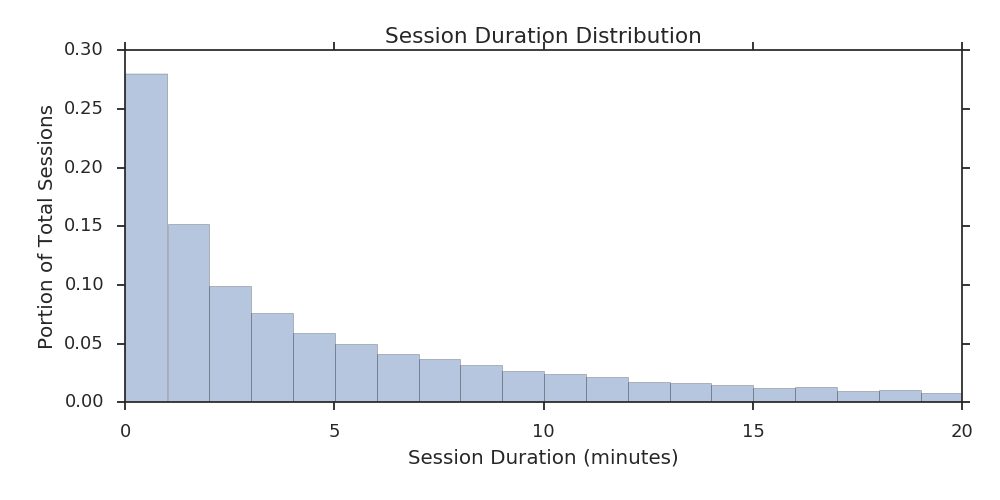
\includegraphics[height=2.75in]{SessionDurationHistogram_v1}
\caption{A histogram of session duration times in minutes.  More than 1/4 of all sessions are just one minute or less.}
\label{fig:SessionDurationHistogram}
\end{figure}

At present, there are separate IOS and Android apps for each of eight titles in subjects including Anatomy and Physiology, Medical Terminology, Psychology, Human Resources Management, American History, Majors Biology, Human Anatomy, and Medical Assisting Certification Prep. 

\subsection{User Interface}
    
The StudyWise apps are all native applications specifically written for smart phones, with an IOS and an Android version available for each title.  When a user opens an app for the first time they are asked if they want to register with an email address.  This information is used only to allow the synchronization of a user's progress in the app between two different devices, such as, for example, an iPhone and an iPad or between an Android phone and an iPhone.  There is a hamburger menu in the upper left-hand corner of the screen which allows the user to (a) Study, (b) get Help or (c) Create an account for synching between devices and to also check for updates to the app's content.  

To start a learning session, the user goes to the "Study" page, which gives the app's name at the top of the page and has two modes:  "Targeted" which presents a list of Topics from which the user then choses a topic from which questions will be drawn or "Review" which presents an overall measure of progress through the app and then will present questions from the set of Topics a user has previously studied (Figure \ref{fig:TopicSelect}).

\begin{figure}
\centering
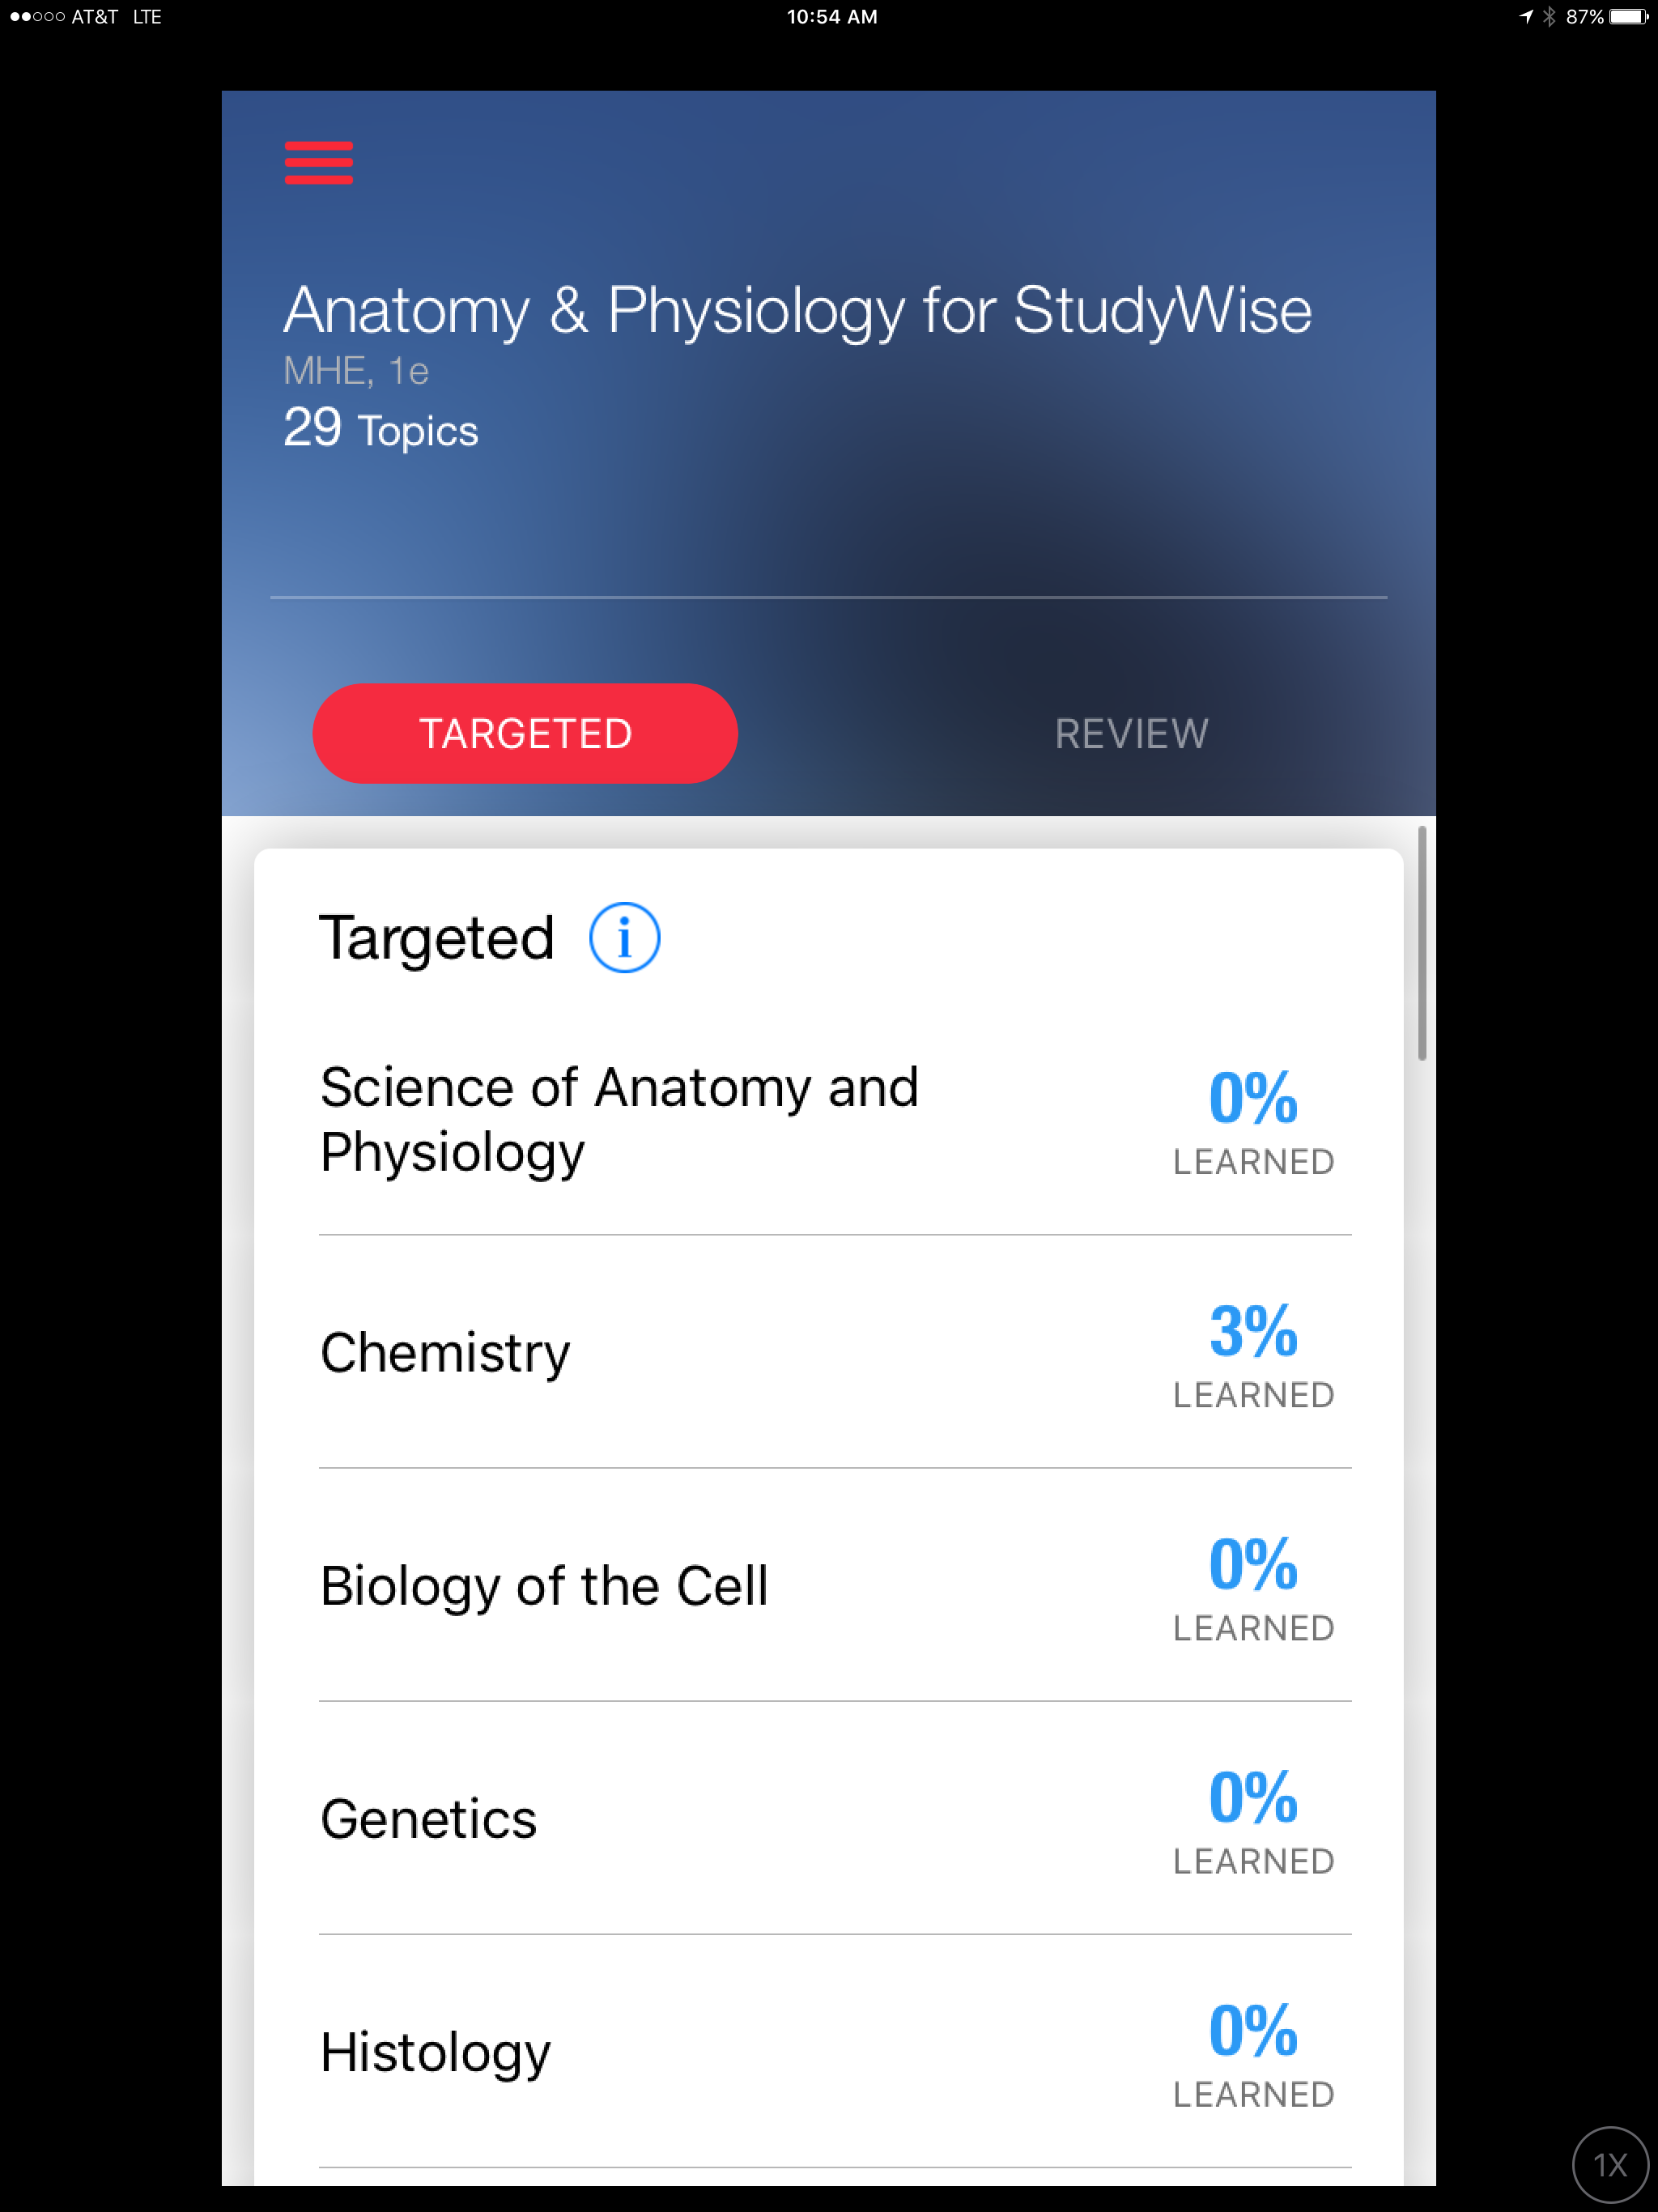
\includegraphics[height=2.75in]{StudyWise_Topic_Selection_Page}
\caption{The Topic selection page for the IOS Anatomy \& Physiology for StudyWise app, with Targeted mode selected.}
\label{fig:TopicSelect}
\end{figure}

Once a topic is selected, the algorithm selects the first LO and one of that LO's probes is then chosen at random.  This first probe is then displayed on the next screen.  The question presented will be one of several types found in SmartBook: multiple-choice single answer (as shown in Fig. \ref{fig:Question}), fill-in-the-blank, multiple-choice multi-answer, matching, matching-rank, or deconstruction (a special type for medical terminology).

\begin{figure}
\centering
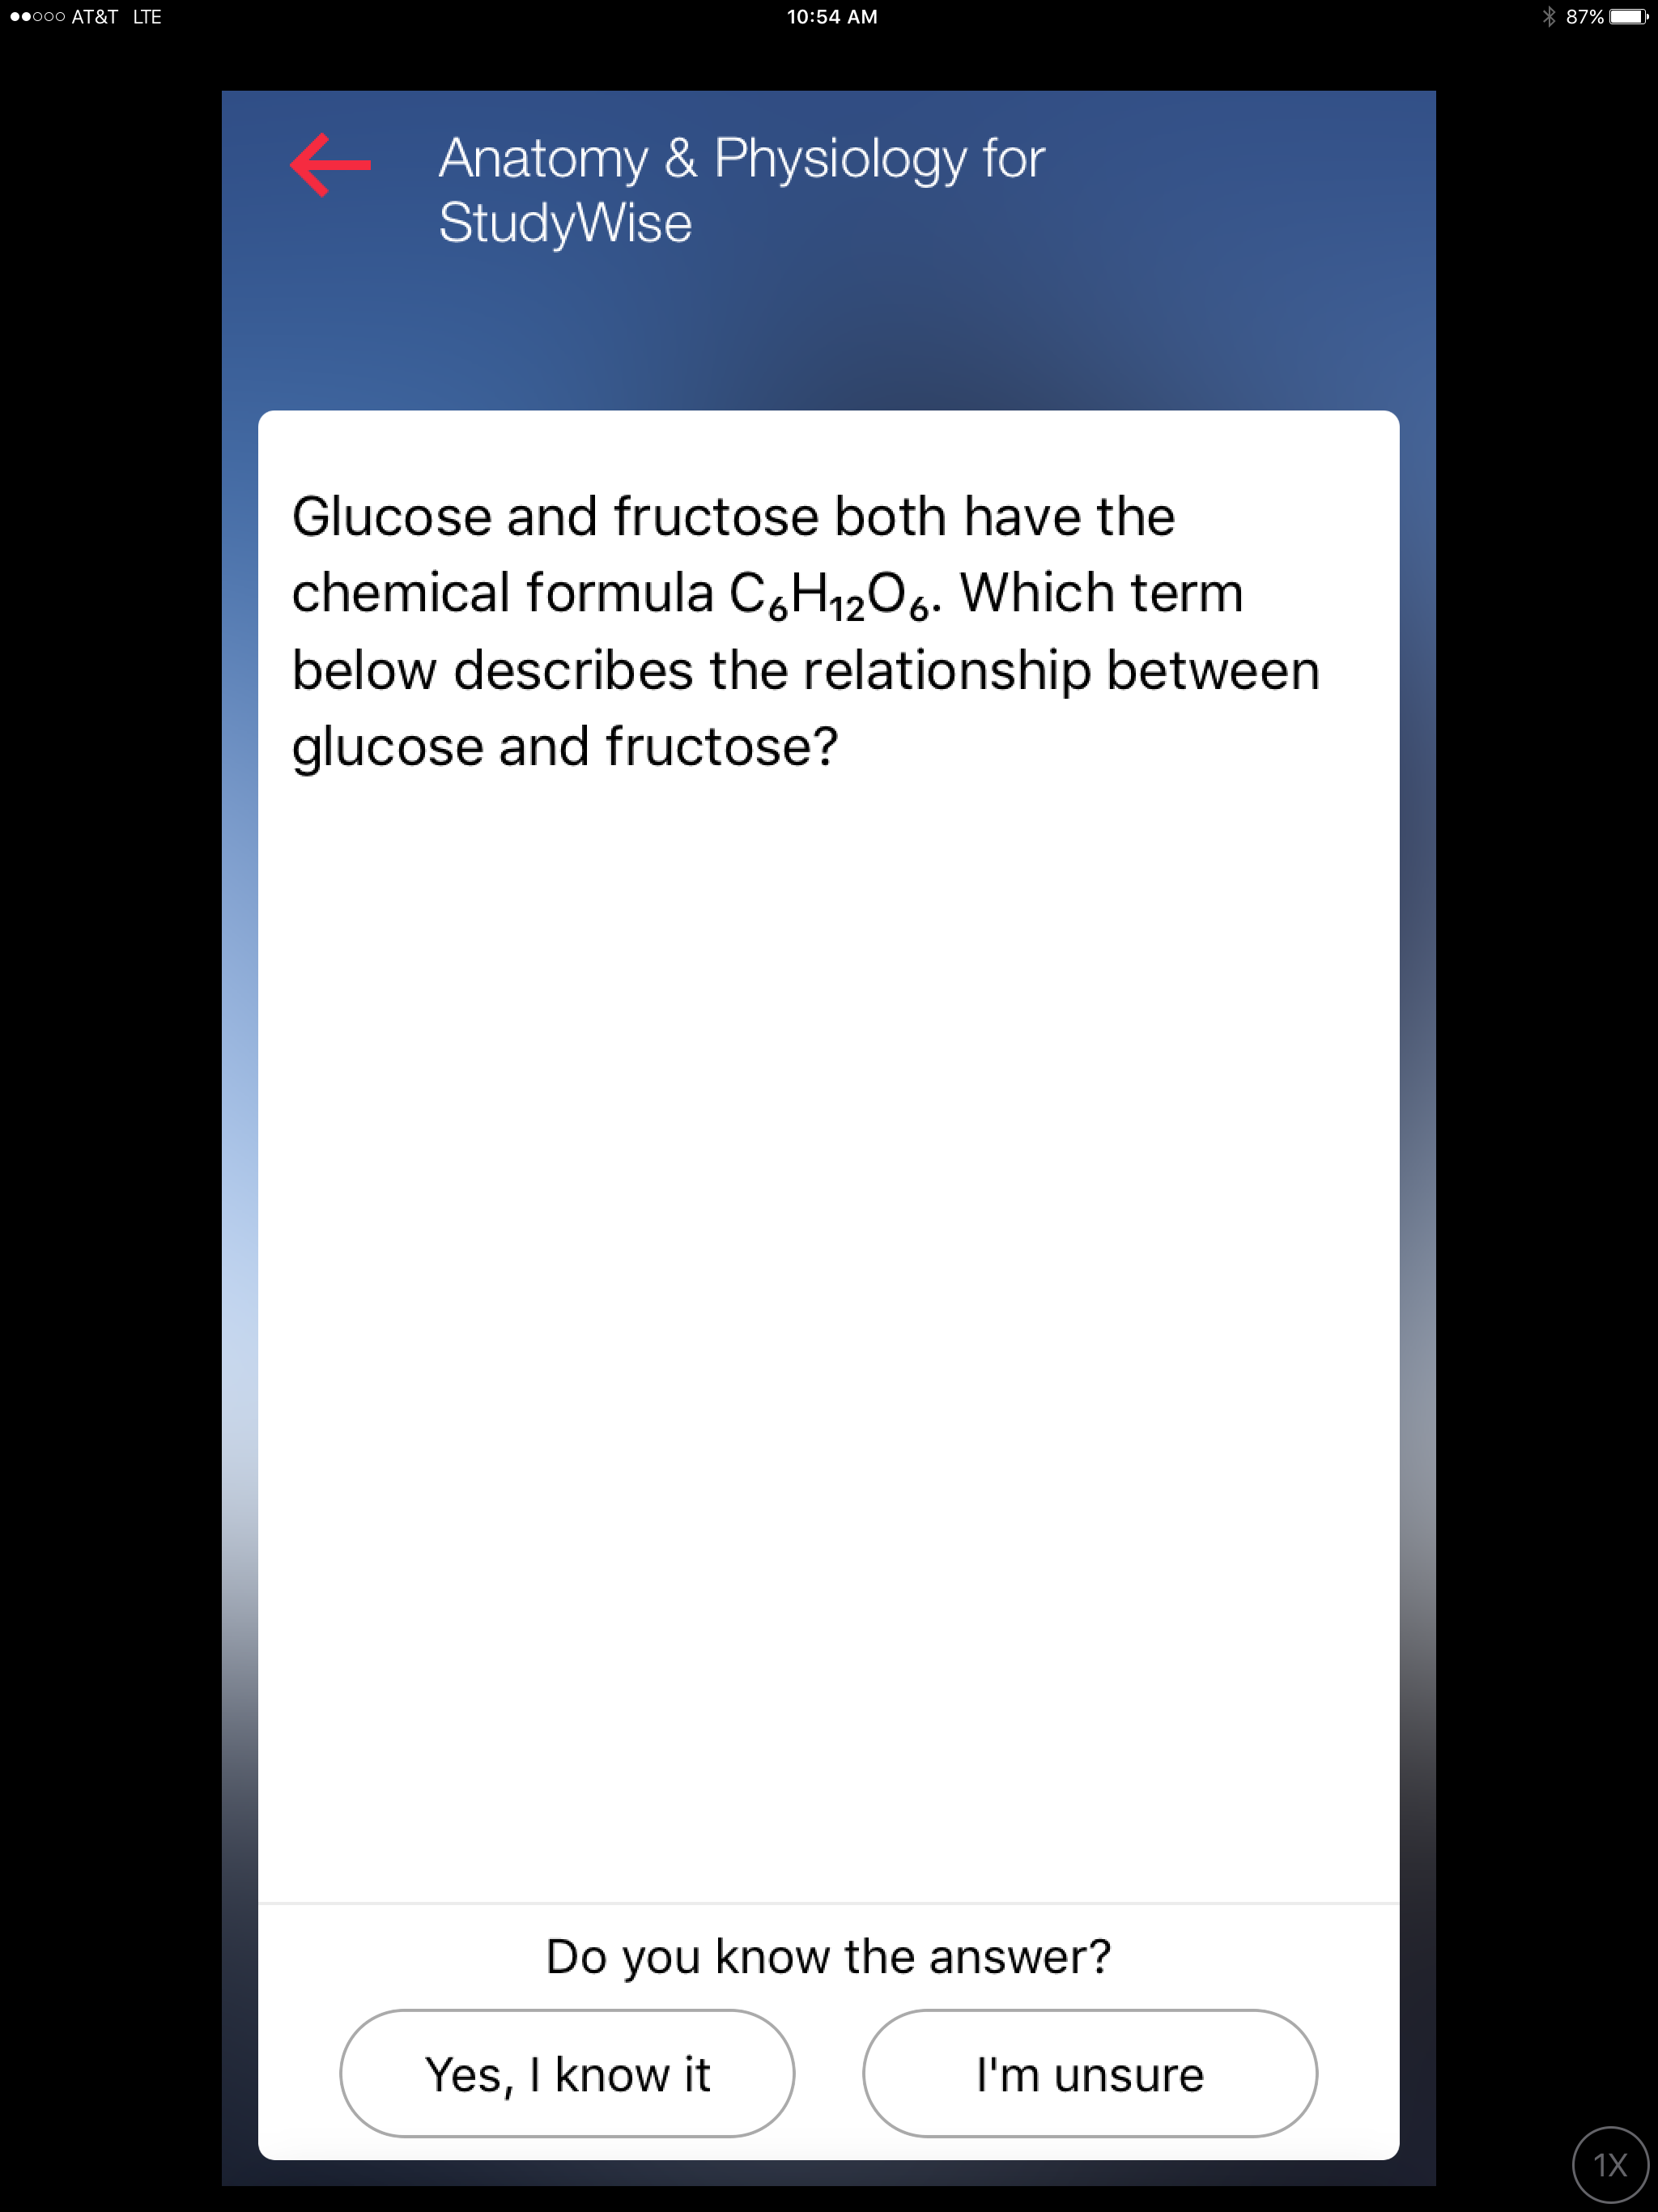
\includegraphics[height=2.75in]{StudyWise_Question_Page}
\caption{The question presentation page.}
\label{fig:Question}
\end{figure}

At the bottom of the page, a question about the learner's confidence about their knowledge of the question appears: "Do you know the answer?", with the two possible choices "Yes, I know it" or "I'm unsure".  The user must answer this question in order to move on to the next page.  For fill-in-the-blank, matching, matching-rank, and deconstruction questions, answering the confidence question submits the answer for grading.  

For multiple-choice single-answer and multiple-choice multi-answer, the next page is the answer selection page (Fig. \ref{fig:AnswerSelect}).  For this case, the user can then either scroll back to the question page and update their confidence after seeing the possible answers (after which the answer page is again displayed) or simply select their answer(s) from those shown.

\begin{figure}
\centering
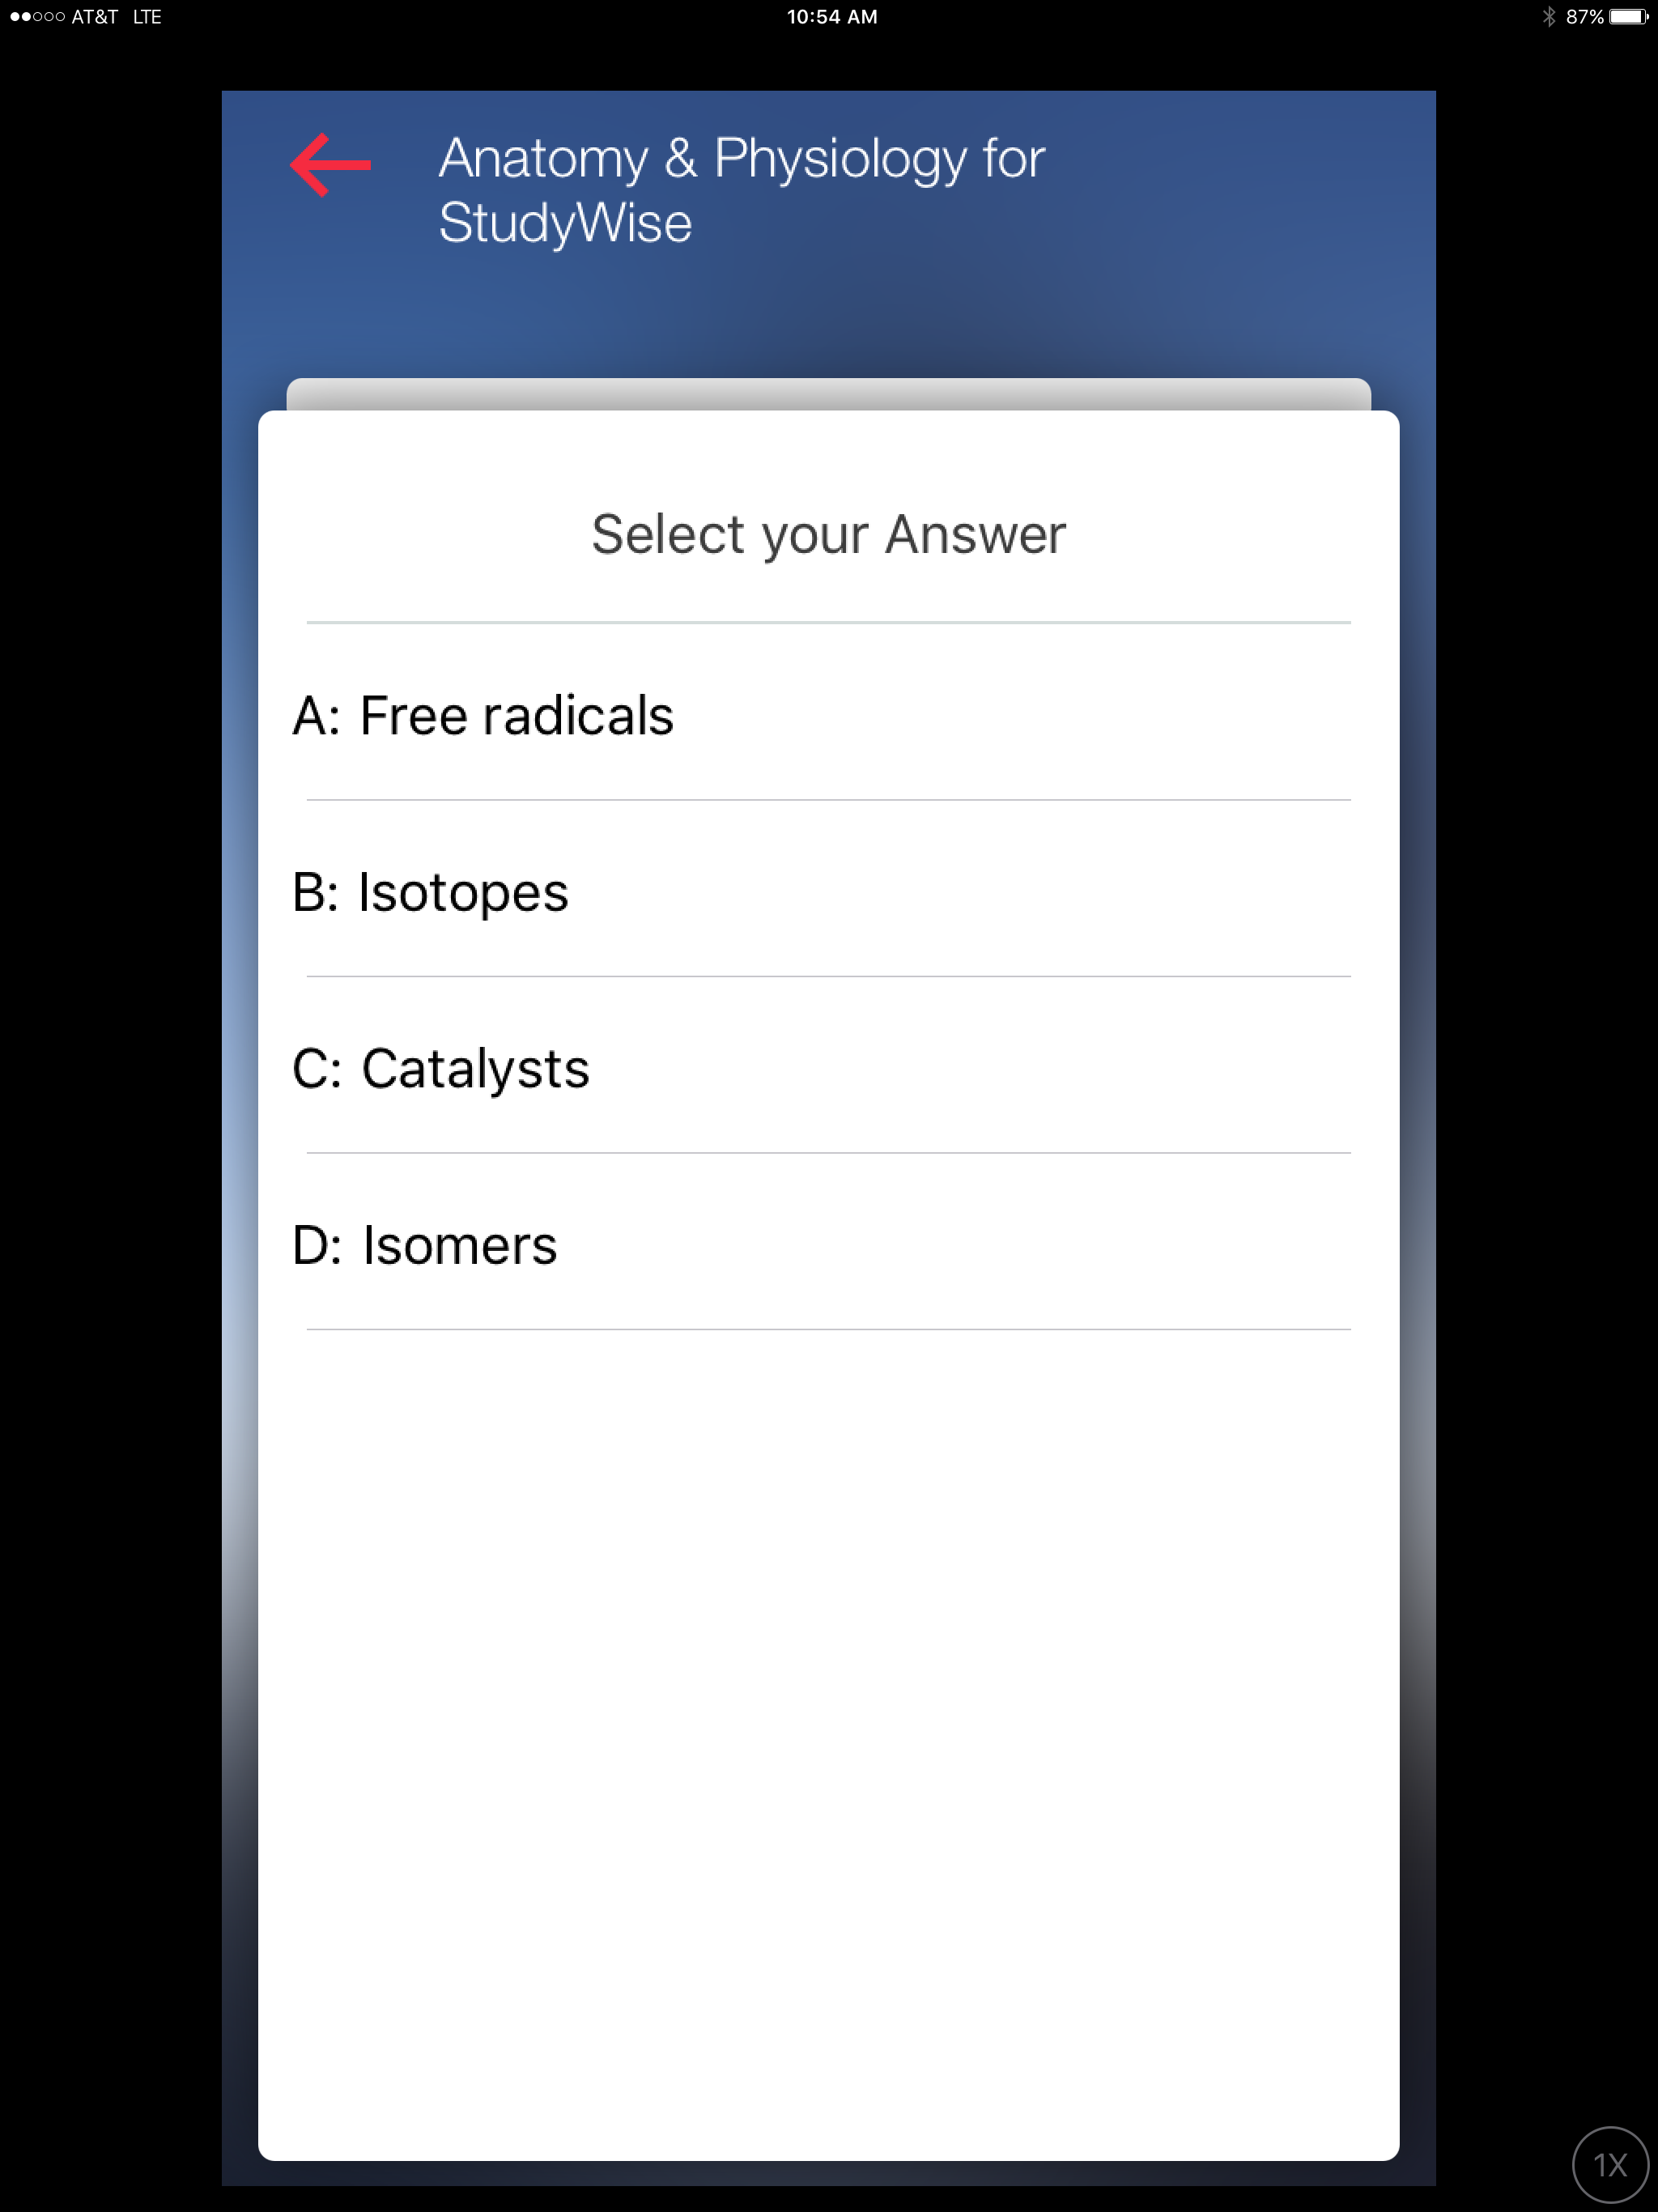
\includegraphics[height=2.75in]{StudyWise_Answer_Selection_Page}
\caption{The answer selection page for multiple-choice questions.}
\label{fig:AnswerSelect}
\end{figure}

Once the user's answer is submitted, the answer is checked against the correct one and an answer response page is then shown (Fig. \ref{fig:AnswerResponse}).  This page reiterates the user's answer and indicated confidence, whether or not the answer was correct, and then gives additional background information on the question's content.  The level of this additional information varies from question to question depending upon how much such background the author of the SmartBook probe included when it was originally created.  

The user then can select the "NEXT" button at the bottom of the page to move on to a new LO's probe chosen by the algorithm or the user can hit the back arrow in the upper left-hand corner to return to the Topic selection page, ending that session.  At that point, the user can again chose a Topic or can hit their device's "Home" button to exit the application.

\begin{figure}
\centering
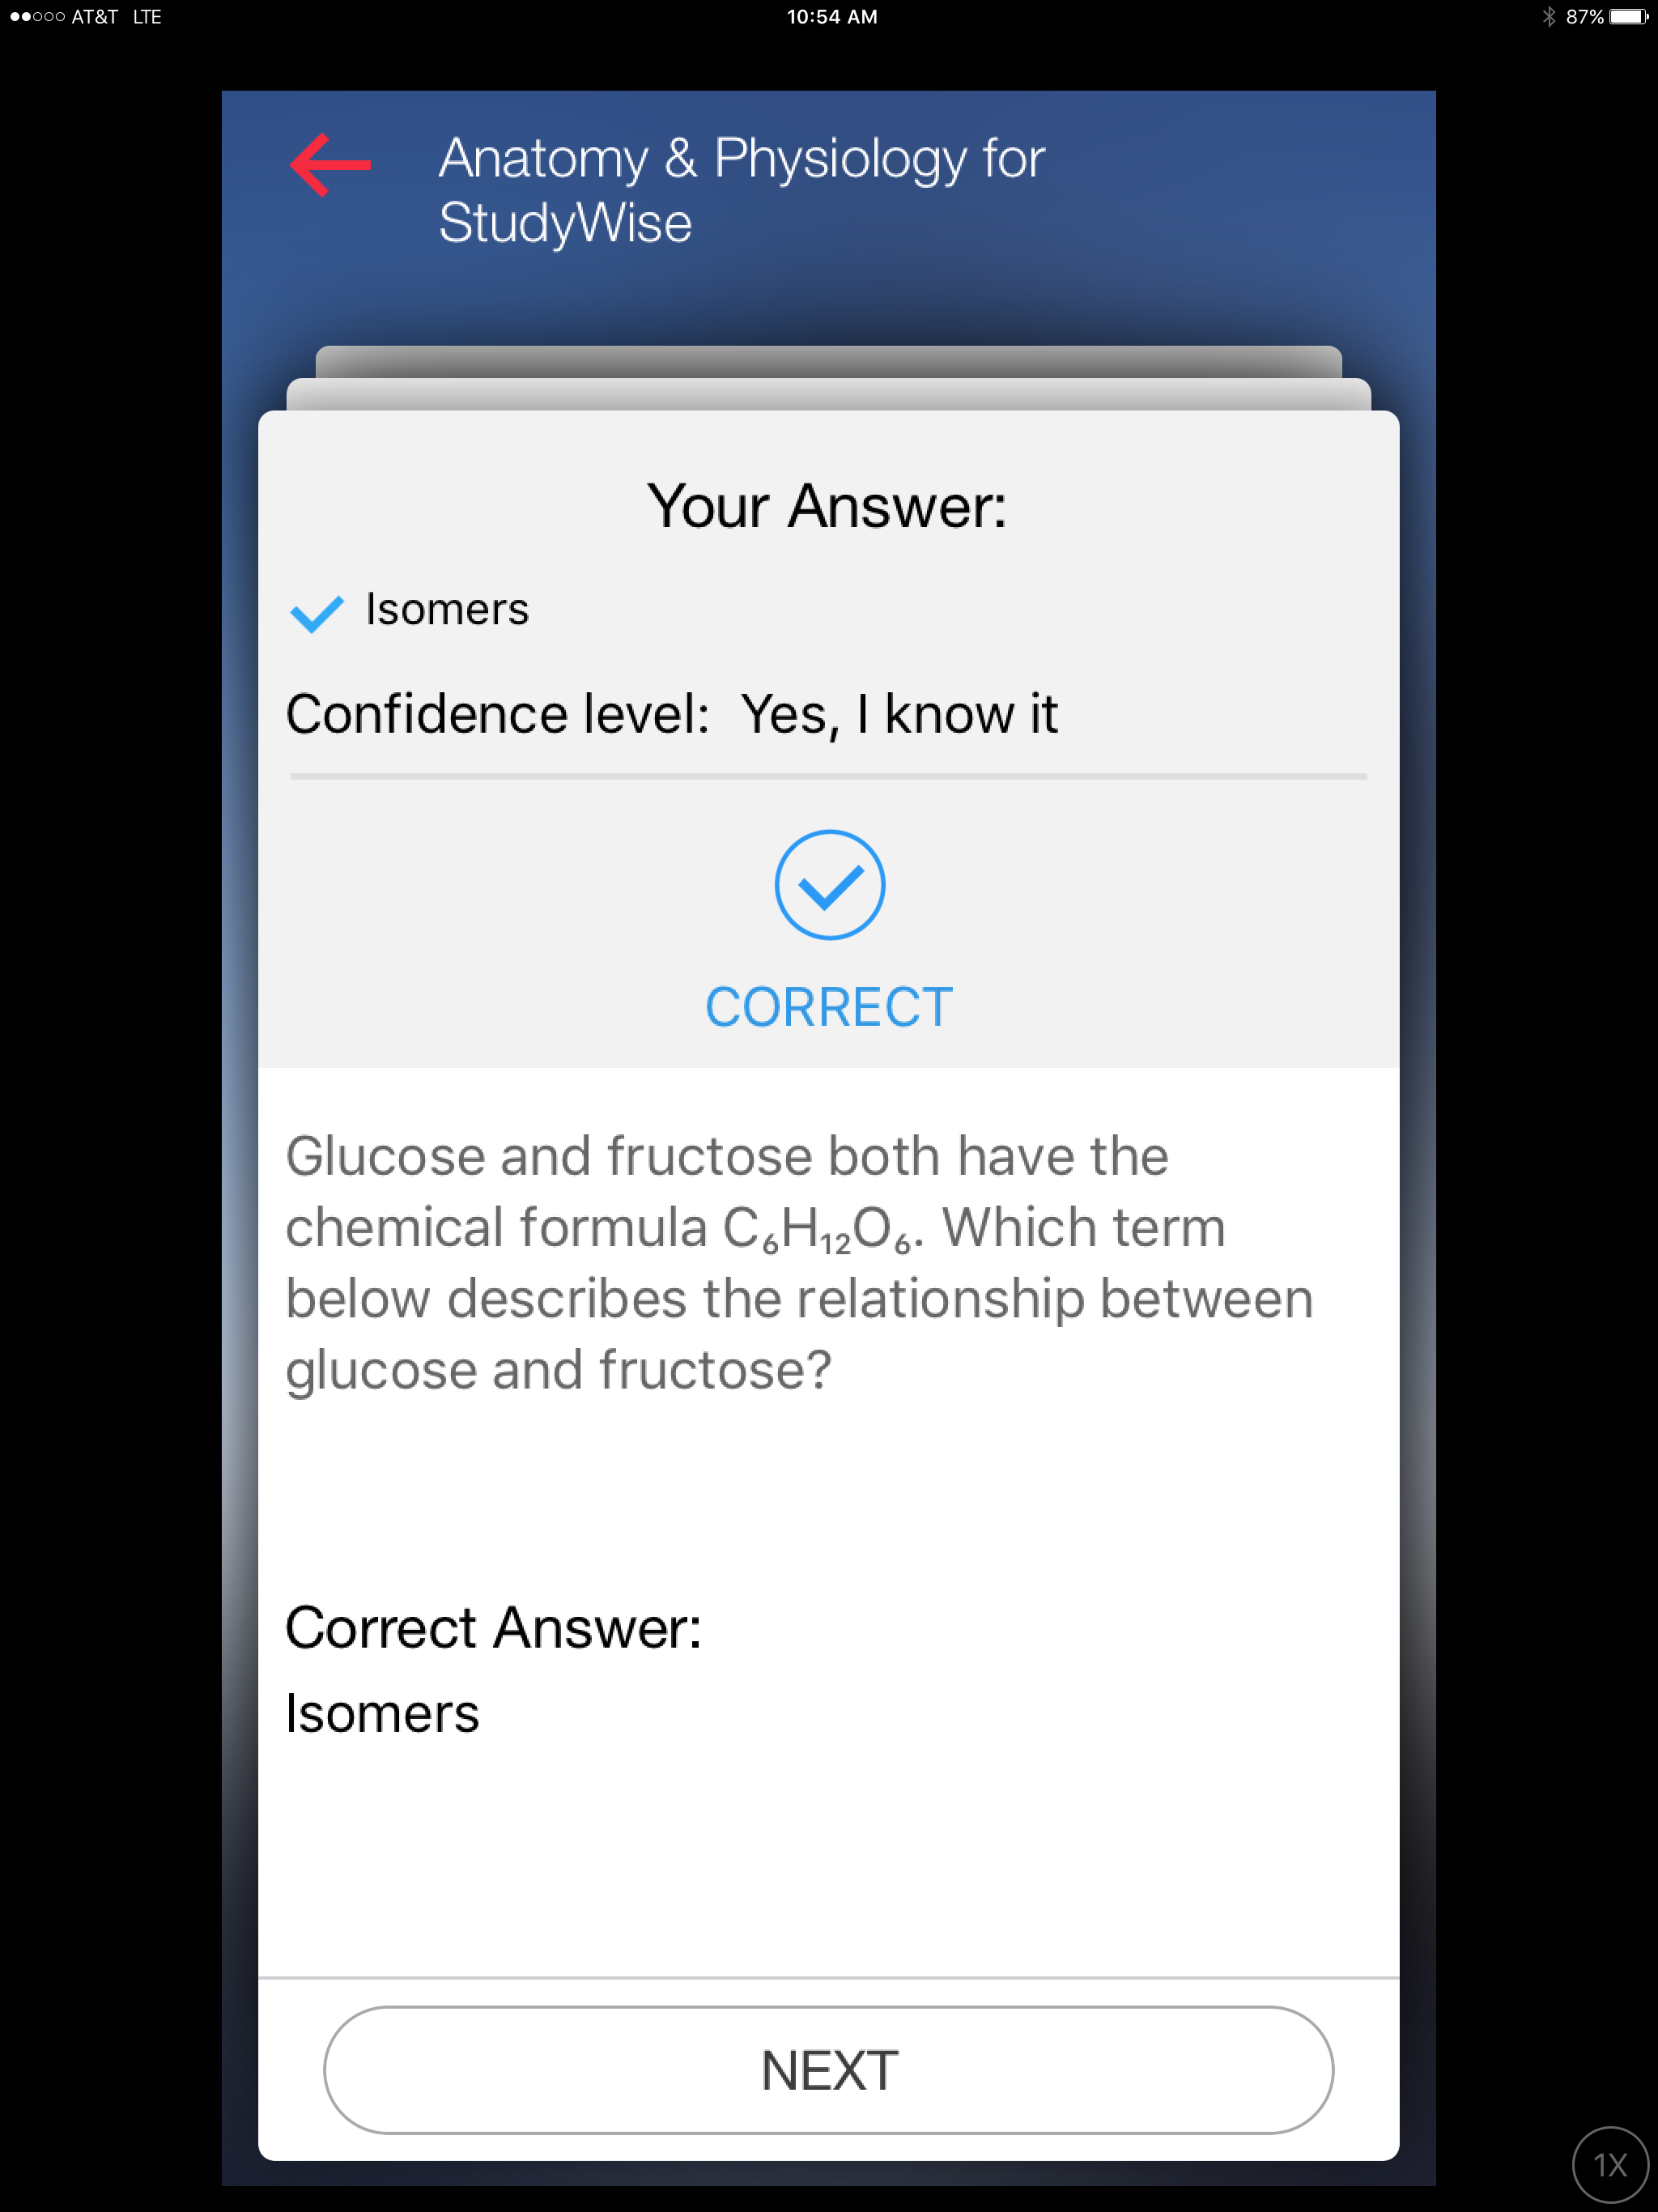
\includegraphics[height=2.75in]{StudyWise_Answer_Response_Page}
\caption{The answer response page.}
\label{fig:AnswerResponse}
\end{figure}
  
\subsection{Algorithm Self-contained within the smart device}   
  
A key element of effective memorization is repeating an item often enough for it to be remembered.  However, we do not want to waste the learner's time by repeating items already well learned.  The algorithm used in StudyWise is a proprietary one with uses a mathematical algorithm which has adjustable parameters that vary the appearance time of the questions associated with each LO.  This spacing also depends on whether or not an LO's previous question was answered correctly or not, if this was not the first appearance of that LO.  For an LO to be considered learned, a total of three correct answers to that LO's associated questions is required.

When an LO first appears, it will be repeated frequently until the first correct answer is given.  After this, the LO is repeated somewhat less frequency, and after a second correct answer, the repetition interval is lengthened even more.  The spacing also depends on the number of LOs included in a given topic.  The desired practice schedule was specified by subject matter experts, who wanted topics of a particular size to fit within a specified practice schedule.  A sample pattern of LO appearances with time is shown in Figure \ref{fig:30_From_100LOs}, for a Topic with 100 LOs  \cite{Riedesel2017}.

This algorithm is compact in both size and computational complexity and is easily self-contained within a learner's smart device.  The learner's complete record of progress through each topic within a title is also stored locally.  This means that the full adaptive experience can be presented to the learner even when not connected to the internet.  A learner can practice for hours, days, weeks, or even months without a network connection.  This was originally motivated by the desire for medical students in rural India to be able to use this application but it also means that it can be used seamlessly even on an airplane flight or other locations where cellular data service is not available.

\begin{figure}
\centering
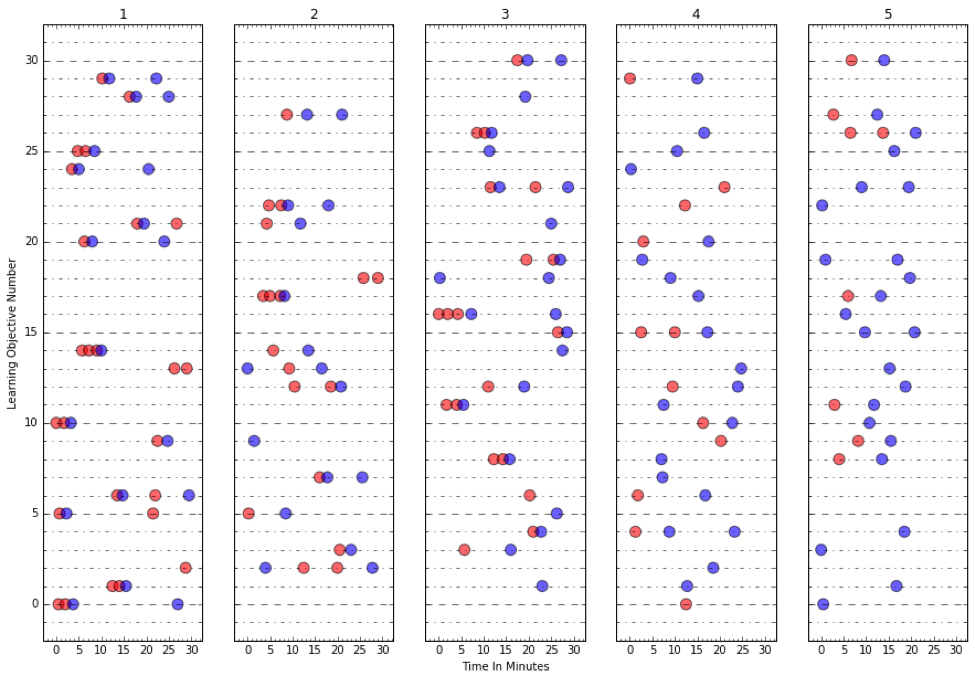
\includegraphics[height=2.75in]{30_From_100LOs}
\caption{Plots of the first 30 LOs from a 100 LO deck. Five 30 minute sessions were
needed to complete 100 LOs. Red dots indicate incorrect answers, as computed by
the model, and blue dots are for correct answers. The start times for the sessions are
separated by 24 hours.}
\label{fig:30_From_100LOs}
\end{figure}

\section{Data Messaging System}

The availability of cloud-based computing and storage allows a smart device to return information on user interactions with StudyWise apps without the need for a database to present the user interface or to store data messages produced by user interactions.  In this way, smartphones hosting StudyWise operate in the same way as devices which are part of the Internet of Things (IOT).  The particular architecture used for StudyWise is based on Amazon Web Service's "Serverless Computintg" technology [\url{http://aws.amazon.com/serverless/}], which is frequently employed for IOT systems. 

This architecture works very well for applications which are designed to stand alone on a user's smart device, and it is also at the heart of how internet-connected sensors and devices which are part of IOT return the data used in machine learning and other predictive analytics.  Using this type of architecture, as noted, there is no database behind the application.  This means that the usual methods of doing both business and educational analytics by querying relevant data from an OLTP database are not available.  All of the data that business analysts and learning scientists use must come from a custom designed system of messages which are sent as learners interact with the system.  

When designing the messaging system we solicited input from both  from the business owners of the application and from  learning scientists.  We wanted to ensure the availability of the data needed for an understanding of the frequency and patterns of use needed for business analytics and for doing the Learning Science related to spaced practice and active retrieval.  Both types of information can be used to improve the user experience and the educational effectiveness of this suite of applications.  

By design, as little personally identifiable information (PII) is ever solicited from the users as possible and none is transmitted to the data collection system.  The only PII information StudyWise uses is the email address used to synchronize a user's progress between devices.  Even this information is contained in the JSON messaging data only as a non-reversible hash of the input email address.

\subsection{Questions for business analytics}

To determine what data might be needed for business analytics, we asked the Higher Education group for a list of the type of reports they might want to be able to construct from the messaging data.  They provided a list which guided our design.

Here are some examples of the types of questions the business analysts wanted to be able to address: 
\begin{itemize}
\item  How much was each application used in terms of questions answered per unit of time (hour/day/week/month)?  
\item What is the pattern of usage in terms of time of day, in local time? 
\item How is usage correlated with the time of year, such as the start, middle, or end of a semester?  
\item How many learning objectives have been answered for each topic for each title?  
\item What is the average user progress through each topic?  
\item What is the usage for IOS vs. Android for each title? 
\end{itemize}

One field added specifically to address some of the business questions was the local time zone, in terms of offset from UCT.  

\subsection{Questions for Learning Science}

In addition to data for business analysis, we also wanted to be able to measure the efficacy of the apps and to be able to gain insight into the learning science related to spaced practice and active retrieval.  To be as comprehensive as possible, we consulted with the MHE Data Science team and with academic learning scientists while defining the messaging fields.

Among the types of questions we would like to be able address in this area include:
\begin{itemize}
\item  Which app (i.e. which Title) is the learner using?
\item Which Question (including its Topic and Learning Objective) has just been answered?
\item Which answer was selected and was it the correct answer?
\item How long did did it take to answer the question?
\item  How long was spent looking at the explanation of the answer?
\item What do the learning curves look like for each learning objective and or each student?
\item What confidence level was chosen and how does it correlate with the correctness of the answer?
\item How do performance and confidence vary as a given LO is repeated?
\item How far through a given topic has the user progressed?
\end{itemize}

\subsection{Data Fields and JSON Schema for the Messaging System}

To be able to answer all of the above questions, the data fields in Table \ref{table:AnalyticsAPI} were created.  There are also several fields to identify the  version of each app overall and the version of the adaptive algorithm which are not shown in this table.  As the application is in use, each time an answer to a question is submitted, information is sent.  Fields which are directly linked to a user's practice session come from the  StudyWise "App" and those which give information on the user's device, time zone, and other information on the session's context come from the mobile devices "Mobile OS" and hardware.

Although both IOS and Android mobile devices can transmit a user's location, the business owners were concerned that asking the user for permission to include their location would be seen as unnecessarily intrusive and might also raise student privacy issues, so this information is not collected.  Local time zone information is collected for determining the time of day an app is being used.

\begin{table}[h]
\small
\caption{Data Messaging Schema}
\begin{center}
\begin{tabular}{ | l | l | p{7cm} | l | }
\hline
Item & Type & Example & Source \\
\hline
IOS Version Number & string & 9.0.1 &  Mobile OS \\
\hline
Device Type & string & iPhone 6+ &  Mobile OS \\
\hline
IP address & string & 10.10.10.10 & Mobile OS \\
\hline
Studywise Application & string & A\&P & App \\
\hline
Software Version	 & string & 1.0.0 &  App \\
\hline
Algorithm Version & string & 1.0.0 & App \\
\hline
Topic IDs & string & [224562,135283,252034] & App  \\
\hline
Topic Titles & list string & ["Countries and Capitals","Present Tense Irregular Verbs","Past Tense of Verbs"] &  App   \\
\hline
StudyWise Topic Size & number & 68 &  App  \\
\hline
User ID & string & 315352FD-44B1-406E-A785-B74100A0B2A9 &  App \\
\hline
Session ID & string & 3B20792D-F46B-48B4-8F45-AA79AE620EA	 &  App  \\
\hline
Date/Time Session Start & string & 2015-08-01T06:00:00.000Z &  App \\
\hline
Event Type & string & one of "targeted" or "review" &  App \\
\hline
Learning Objective ID & string & CL323778e1-8d23-425f-8be4-996f20ae4933 &  App \\
\hline
Question Identifier & number & 589823749 &  App  \\
\hline
Question Type & string & multipleChoice/MCQ &  App   \\
\hline
Date/Time Presented & string & 2015-08-01T06:00:00.000Z & Mobile OS \\
\hline
Date/Time Answered	 & string & 015-08-01T06:00:00.000Z &  Mobile OS \\
\hline
Answer Selected & string & CL323778e1-8d23-425f-8be4:243565606:0 &  App. \\
\hline
Success/Failure & number & 0 for failure, 1 for success &  App \\
\hline
Confidence & list & 1 or 2 [1, 2] & App \\
\hline
User Interrupted Details & list or string & [ "phone", "other" ] & Mobile OS \\
\hline
Session Progress & number &  53\% & App  \\
\hline
Product Title & string	 & Anatomy \& Physiology & App \\
\hline
Product Id	 & number & 151514 &  App \\
\hline
Local Time Zone & string & -5 & Mobile OS \\
\hline
Date/Time Session End & string & 2015-08-01T06:00:00.000Z & App \\
\hline
\end{tabular}
\end{center}
\label{table:AnalyticsAPI}
\end{table}


\subsection{JSON schema}
   
JSON was specified by MHE's data engineering group for encoding the messages in order to be compatible with a company-wide standard for data messaging systems for future educational software products.  IMS Caliper was considered as the basis for this API, but at the time this API was designed (in mid 2016) Caliper lacked a number of fields needed to satisfy both the educational and business requirements, and MHE's data architects approved the schema shown here.

One great advantage of using JSON is the ability to query a collection of JSON documents using standard SQL query commands.  This can be done either through systems such as Apache Spark [\url{http://spark.apache.org}], jQuery [\url{https://jquery.com}], or other similar tools.  Even quite complex queries have worked successfully and an experienced database analyst can fully leverage their background in the SQL language while analyzing this type of data.  In analyses done thus far, essentially all SQL queries attempted using Apache Spark SQL have worked on this data set. 

\subsection{On-line and off-line modes}

The first version of StudyWise was created to allow medical students overseas to study for the United States Medical Licensing Exam (USMLE).  Such students could possibly be in areas where network coverage was spotty, so StudyWise was designed to be fully usable when the user's mobile device was had no cellular data connection.  This means that all of the logic and code needed for a fully adaptive experience needed to be contained in Javascript code on the mobile device.  Similarly, all of the questions, answers, explanations for incorrect answers, and ability to determine if an answer was correct or incorrect is included in the mobile app.

However, it was still desired to have a record of user interaction data, even for sessions done off line.  In order to accommodate this, the JSON analytics data message for each interaction is either (1) buffered and then sent to the collection server in MHE's AWS virtual private cloud (see below) if the user is connected or (2) stored locally on the mobile device for later transmission if a network connection is not currently available.  Stored data from off-line sessions is later sent to the collection server when a user is running the StudyWise app and has a network connection.  At present, this is the only widely available mobile educational application of which we know that has this capability.

\subsection{Receiving system}

As an app is in use, each time a learner answers a question, a JSON record is generated.  This record is stored locally in a buffer and when this buffer is full or the session ends, the buffer of records is securely transmitted to a receiving service running on an AWS instance.  The receiving service validates the data, as described below, and stores it in a flat file in a secure location in AWS S3 file storage.

The storage is a simple directory hierarchy organized by year, month, day, and hour.  Many utilities exist to read JSON data stored in this way, including  in Apache Spark.  As noted above, this type of JSON file system can also be directly queried using SQL just as if it was a relational database.

This method of collecting and storing the data is limited in speed by the transmission time of the internet but otherwise is capable of very high data throughput and can be set up in parallel to scale almost arbitrarily, if necessary.  Total storage available is essentially limited only by the ability to pay for it.

This means that this data system could handle potentially millions of users daily by simply scaling out the receiving and storage systems, with no change in architecture.  Using the capabilities of AWS means that no server or storage hardware need be purchased to set up such a system.

\section{Security and Privacy} 

As a system which is used in education, it is very important to maintain the privacy of each user's data.  This requires an architecture which protects the integrity and security of the data at each step of the collection and analysis.  An important first step, as noted above, is to store no personally identifiable information in the analytics data stream.

\subsection{Data Encryption}

Data encryption is a critical element of security. Strong encryption of data both at rest and in transit prevents an attacker who might gain access to a storage system or communication channel from obtaining sensitive information.  In StudyWise, this means that all communications between the mobile application, the data collection end-point, and the processing pipeline are encrypted using HTTPS/SSL. 

Data stored for analysis, and the derived datasets that comprise the output of those analyses, are encrypted in cloud storage. Amazon S3 supports multiple mechanisms including SSE-S3 (transparent server-side encryption), SSE-KMS (server-side encryption using AWS key management) and SSE-C (server-side encryption using customer-provided keys).

Furthermore, the pipeline runs in a virtual private cloud on infrastructure not directly accessible from public networks.

\subsection{Access Policies and Controls}

User authentication controls who can access the analytics environment. Integrated identity management can simplify user management by leveraging a service to authenticate users.  Examples include SAML2.0 and Active Directory.  

In order to ensure that only authorized users can access data stored and processed in the analytics pipeline, role-based access provides fine grain controls on storage (who can access data sources in the processing environment), on clusters (who/what is authorized to configure/launch/terminate/restart clusters) on processing jobs (who/what can attach and run processing on clusters) and the environment (configuration and settings).

Auditing and logging provide the ability to alert on, monitor, and review key events in the environment.

\subsection{Data Integrity}

In the compute layer, within Apache Spark, the RDD (see below) provides data immutability and fault-tolerance by design. In the storage tier, AWS S3 provides not only an extremely high level of durability (99.999999999\%) but also the ability, via the optional Content-MD5 request header, to verify the integrity of data stored there.

\subsection{Certifications}

An end-to-end data analytics pipeline, especially one reliant on third-party managed or cloud services, is a system based on the integration of many components. No matter how strong the data encryption and access policies in place, the system is only as secure as its weakest link. Managed service and cloud providers certify their platforms according to documented compliance standards. 

The FERPA (Family Educational Rights and Privacy Act) standard governs access to educational information and records. Other standards, many originating in the financial and health industries, are also relevant in education.

AWS documents their compliance at \url{https://aws.amazon.com/compliance/}. Certifications include FERPA, HIPPA, GLBA, FISMA, RFR, and PCI DSS.

Databricks, the computing environment used here for data analysis, documents their platform security and compliance at \url{http://go.databricks.com/}.  Their security measures are based primarily on SOC2 Type-1 Certification. SOC2 Certification encompasses 5 key areas: security, availability, processing integrity, confidentiality, and privacy.
    
\section{Data Processing and Analysis}

In order to use the data collected for either educational or business insights, we need to set up a system to read, clean up, and analyze the JSON data produced originally on each user's device which has been sent to the AWS S3 collection system.  It is possible to do all of this entirely in the cloud using AWS and other services and this is the approach that we have taken with StudyWise.

In particular, we would like a system which has the following characteristics:  (1) straightforward to access, use, and maintain and (2) powerful and scalable enough to handle increasing amounts of data as StudyWise is more widely deployed.  In the past ten to fifteen years, several systems have been developed which have been designed to satisfy these type of needs.  All are based on horizontally scalable clusters of servers to allow computing to be done in parallel.

Many high performance computing systems in use by the academic and government research communities use the Message Passing Interface (MPI) to do parallel computing.  This requires writing code in either C or Fortran.  This is scalable to the very largest systems in existence and can be used for the most complex types of parallel computing but it requires a very high level of specialized knowledge and expertise to use.  MPI can be used not just for processing large amounts of data in parallel but also for doing very large parallel theoretical calculations for such applications as global climate models and modeling the interiors of stars.

A system designed to make parallel computing more accessible to a wider range of users is the Apache Hadoop/MapReduce system of software developed for the parallel processing of large amounts of data.  This system is simpler than MPI but still requires the use of the Java programming language and also requires writing intermediate results in its processing pipeline to disk, which can make it rather slow.

To overcome the limitations of MPI and Hadoop/MapReduce, a system called Apache Spark [\url{http://spark.apache.org/}] has been developed by the open source community which allows all of the computation to be done in a compute node's memory and which also combines some of the steps in map/reduce processing, making the writing of code to process large amounts of data in parallel considerably easier than previous systems.  Apache Spark has come into wide-spread use in just the last three to four years but is becoming the dominant method of processing very large amounts of data.  

Spark also is available with APIs for programming in Scala, Python, R and SQL, making it accessible to a much wider audience.  On a practical level, a Spark program can be many, many times faster (x100, in some cases) than an equivalent Hadoop/MapReduce program, as long as all of a given sub-set of data in a parallel processing job can be fit into the memory of one of the servers in a Spark computing cluster.

In this section, we show how Apache/Spark can be used to process and analyze large scale data with examples of its use in StudyWise.

\subsection{Apache Spark}

Apache Spark is both an engine and API for large scale data processing, making very large scale parallel computing accessible to a much wider range of users than previous parallel computing methods.  Large organizations have deployed Apache Spark on clusters consisting of thousands of nodes, processing petabyte sized datasets which grow on the order of terabytes per day \cite{Tsai2017}.

The main abstraction in Apache Spark is the RDD, or resilient distributed dataset.  

"Resilient" refers to redundancy of data across compute nodes, Apache Spark's fault-tolerance and ability to continue processing when compute nodes fail. 

"Distributed" refers to the fact that data is partitioned across many multiple cluster nodes. More importantly, computations are moved to the data, rather than the traditional approach of moving data to central location(s) for processing. This eliminates I/O bottlenecks and allows processing to scale in a linear fashion as the amount of data grows.

"Dataset" refers to large scale collections of data. An important attribute of these datasets in Apache Spark is immutability. Immutability drastically simplifies the cost and complexity of coherently processing distributed data. Spark represents processing steps in a directed acyclic graph. This traversable graph, combined with the immutability of data at each intermediate step in the process, allows datasets to be easily reconstructed on failure, contributing both to the resiliency and distributed characteristics of the system.

More recently, Apache Spark has added an additional abstraction layer on top of the RDD called a dataframe.  The dataframe makes the manipulation and processing of the data conceptually simpler than is the case for RDDs and it is very similar to dataframes found in Python Pandas and in R (where the concept was first developed).

\subsubsection{Data Streaming}
  
Apache Spark supports both batch-oriented and stream processing using a single unified API.  The use of streaming allows essentially up to the second processing to be done on the analytics data as it arrives from the users mobile devices, if desired.

The Apache Spark Structured Streaming API mimics the Apache Spark batch API, but behind the scenes it utilizes the SparkSQL engine to continuously update data as new information arrives. The same SparkSQL queries and operations that work on batch loaded information can also be performed on streaming dataframes.

In the concrete examples below, Spark Structured Streaming is used to perform event-driven processing.

\subsubsection{APIs and Analysis Tools}

Apache Spark's processing API supports multiple languages, including Scala/Java, Python and R as well as a dialect of SQL.  In the following example, data is ingested into a Spark dataframe. Here are brief examples of how to read JSON flat files into a Spark dataframe for the different Spark languages:

\begin{lstlisting}[language=Scala, basicstyle = \small, caption={Scala}]
 val eventSampleDf = spark.read.json("pathBatch/*.json")
\end{lstlisting}%
\begin{lstlisting}[language=Python, basicstyle = \small, caption={Pyspark (Python)}]
 eventSampleDf = spark.read.json("pathBatch/*.json")
\end{lstlisting}
\begin{lstlisting}[language=R, basicstyle = \small, caption={SparkR (R)}]
 eventSampleDf = read.df(sqlContext, "pathBatch/*.json", "json")
\end{lstlisting}

The Apache/Spark API also allows SQL-like operations to be performed on dataframes.

A simple select/filter operation in scala using the SparkSQL API:
\begin{lstlisting}[language=Scala, basicstyle =\small, caption={SQL query using Scala}]
 val apDf = eventsBatchDf.
                     filter($"session.studywiseApplication" === "A&P")
\end{lstlisting}%
The same operation expressed in Spark SQL syntax:
\begin{lstlisting}[language=SQL, basicstyle = \small, caption={SQL query directly in Spark SQL}]
  %sql select * from apDf where session.studywiseApplication = 'A&P'
\end{lstlisting}%


\subsection{Processing Pipeline}

Pipelines typically have at least three layers: input, processing and output.  These are shown in Figure \ref{fig:Pipeline}.

In StudyWise, these layers coordinate with software components that facilitate user authentication, data collection, transmission, and persistence. 

\begin{figure}
\centering
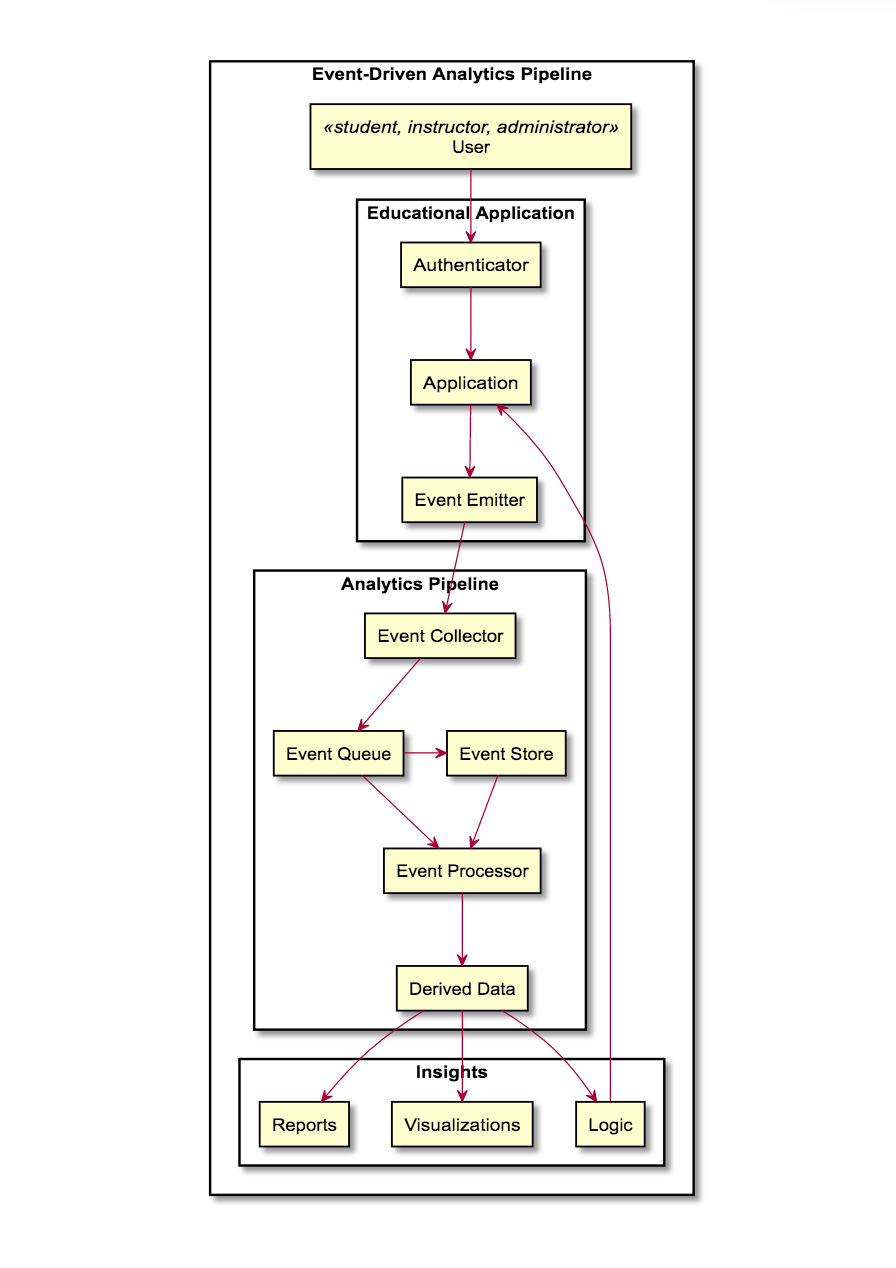
\includegraphics{AnalyticsPipeline}
\caption{The Processing Pipeline for Analytics Data for the Mobile Apps}
\label{fig:Pipeline}
\end{figure}

\subsubsection{Layers of Processing}
\subsubsection{Ingestion via messaging system}

The input layer is preceded by event hooks instrumented in the client mobile application. These event hooks trigger calls to REST APIs that authenticate the user and transmit events to an event collector and cloud-based storage.

Once these events are persisted (in AWS S3, for example), the Apache Spark datasources API can be used to ingest the events into a dataframe for processing.

The Apache Spark API supports both batch and streaming semantics via the same interface.

Read all events in a bulk batch read:
\begin{lstlisting}[language=Scala, basicstyle = \small, caption={Batch Read of a JSON file}]
 val eventsBatchDf = spark.read.schema(schema).json("path/*.json")
\end{lstlisting}%

Stream events as they arrive via streaming.
\begin{lstlisting}[language=Scala, basicstyle = \small, caption={Streaming Read of a JSON input stream}]
 val eventStreamDf = spark.readStream.schema(schema).json("path/*.json")
\end{lstlisting}%

In the case of a batch read, all source events presented at the time of the read operation will be read in a bulk read operation and stored in an Apache Spark dataframe. 

In the case of the streaming read, all source events present at the time of the read operation will be initially loaded into the target dataframe. The dataframe is unbounded, however. As new events arrive, new rows are added to the dataframe.

\subsubsection{Data Cleaning and Transformation} 

Cleaning and transformation consists of Apache Spark and SparkSQL operations on the source dataframe. As discussed, dataframes in Spark are immutable. Every operation on the dataframe creates a new dataframe. Operations are distributed across the worker nodes in the cluster.

\begin{lstlisting}[language=Scala, basicstyle = \small, caption={Filtering out unwanted data fields}]
  // filter out events based on criteria, 
  // in this case columns not used in the processing
  
  val v2Df = eventsStreamDf.drop("legacyData")

  // use SQL-like syntax to group events based on some criteria
  // in this case, by application and product title
  // counted and sorted
  // to produce a continuously updated dataframe containing 
  // the most common application/title combination
  
  val activityByProductTitlesandApplicationStreamDf = 
    v2Df
      .groupBy("session.studywiseApplication", "session.productTitle")
      .count
      .sort(desc("count"))
\end{lstlisting}%

\subsubsection{Intermediate Storage}
Whether transforming data for subsequent analysis, or producing a set of potentially valuable insights, it is useful to persist these results. The Apache Spark datasources API can write the data back into S3 cloud storage in a variety of formats including JSON or to a more optimized and compact format such as Parquet. These operations can also be performed in batch or streaming modes.

\begin{lstlisting}[language=Scala, basicstyle = \small, caption={Creating a Parquet File from raw JSON data}]
  v2Df
    .writeStream
    .format("parquet")
    .option("path", "targetPath/v2DfStream.parquet")
    .start
\end{lstlisting}%

\subsection{Filtering}

The data stream can also be filtered in order to produce more compact data sets for specific types of analysis and also to clean up the data.  For example, during the test phase of the initial StudyWise deployment, the apps would sometimes produce duplicate records.  By applying a filter to the stream, these duplicates can be eliminated.  Other minor data issues have also been filtered out in a similar way.

Is is also possible to filter the data based on any of the data fields in Table \ref{table:AnalyticsAPI}.  A common filter used is to look at a particular title, type of question, correctness of answer, or level of confidence.  Spark SQL makes the construction and application of such filters to dataframes straightforward.
 
\subsubsection{Time Windowing}

A very common way to want to filter data is by time.  To facilitate this, a daily time stamp is added to the StudyWise data stream.  With this, Spark SQL has a built-in Window function which allows the data to be grouped by user specified time windows, such as hourly, daily, weekly, or monthly using SQL-like command.  Operations of many types can be done within these windows, including calculating moving averages and ranking rows, operations difficult to do with standard SQL.  

We have used SparkSQL Window functions, for example, to look at daily usage of each app and also to prepare data for calculating learning curves.  While these types of calculations can be done by spreadsheets, such as Excel, Spark can do this on many millions or billions of records using parallel computation.

\subsubsection{Versioning}
Versioning components of the pipeline is a useful method for tracking features and compatibility as the pipeline evolves. Versioning applies to API endpoints and message/event schema. Increments to the major version number indicate "breaking" changes while increments in the minor version indicate backward-compatible changes.

An example of a minor version change would be the addition of a new field that can be safely ignored. More drastic changes to an interface, such as a change in structure or names of existing fields, require a major version increment.

\subsubsection{Schema Changes}

By including versioning information in the event envelope, the processing pipeline can programmatically handle disparate versions of message formats through a process of transformation and normalization.
\begin{lstlisting}[language=Scala, basicstyle = \small, caption={Filtering events based on a specific software or message version.}]
  val eventSampleDf.filter($"session.softwareVersion" === "2.1.5")
\end{lstlisting}

\begin{lstlisting}[language=Scala, basicstyle = \small, caption={Defining a function to conditionally process events based on version.}]
// event normalization, scala function
def normalizeEvent(version:String, event: String): String = {
  if(version == "2.0" || version == "2.1") {
  	// transformation specific to v2
  }
  else if(version == "1.0" || version == "1.1" || version == "1.0.1") {
  	// transformation specific to v1
  }
  else {
	// other or unrecognized versions
  }
}
\end{lstlisting}


\begin{lstlisting}[language=Scala, basicstyle = \small, caption={Registering a function as a UDF for event processing in SparkSQL}]
// event normalization, as registered UDF function
val normalizeEventUDF = spark.
			udf.
			register("normalizeEvent", normalizeEvent _)
\end{lstlisting}


\begin{lstlisting}[language=Scala, basicstyle = \small, caption={Applying the UDF to transform events in a dataframe}]
val dfTransformed = 
  dfEvents
    .select(normalizeEventUDF($"session.softwareVersion", $"event", $"*")
\end{lstlisting}

\section{Managed Computing Environments and Cloud Computing}

Managing the infrastructure associated with a processing pipeline can be complex and expensive.

A variety of resources must be managed in a processing environment. These include compute clusters, storage, processing code, recurring jobs, and users. In a secure environment, roles and permissions are enforced to limit access to resources. 

In a self-hosted environment, administrators provision and manage these resources. In a managed environment, the service provider simplifies and automates the administration of these resources.

Each of the resources needed for a processing pipeline can be set up in one of several ways. An organization can do all of this in their own datacenter on their own hardware, with their dedicated staff to manage it.  An alternative is to use cloud services to provide some or all of the storage, computing, and data management using such providers as AWS [\url{https://aws.amazon.com/}] and Azure [{https://azure.microsoft.com}]. 

Similarly, the software, such as Apache Spark, can also be installed, maintained, and managed by an organization's own personnel, either by directly obtaining it from the open-source repository or by using  commercially packaged software distributions, such at HortonWorks [\url{http://hortonworks.com/}] or Cloudera [\url{http://www.cloudera.com/}].

There are also cloud-based providers, such as Databricks [\url{http://databricks.com/}] and Qubole [\url{http://www.qubole.com/}] which provide large-scale computing as a service, with data typically stored in Amazon S3 or on Azure.

Our organization chose to host its storage within its own Virtual Private Cloud (VPC) in AWS and to use Databricks for large-scale data processing and analysis.

\subsection{Databricks}

Databricks offers a managed, scalable, and enhanced cloud implementation of Apache Spark including tools to simplify and automate administration of the environment and also includes a notebook-oriented user interface to facilitate the organization, exploration, and analysis of large data sets.  Among the features Databricks offers includes the following:

\begin{itemize}
\item graphical UI layer
\item cluster and job management
\item  user, role and permissions management
\item  improved scalability, elastic/autoscaling
\item  compute cost optimization
\item  vendor-specific enhancements to the processing pipeline
\item  enhanced security
\item  RESTful APIs for user, job, cluster management
\end{itemize}

\section{Data storage and formatting}

When working with very large amounts of data the specifics of how the data is stored and formatted can have a very large impact upon overall performance.  Using the most efficient methods can greatly broaden the scope and types of analysis which are possible and expand the range of learning science questions which can be addressed.

\subsection{Raw JSON in AWS S3 Cloud Storage}

As the JSON data message packets arrive from each user's mobile device, they are validated and processed by an input server running in AWS and then stored in a flat file hierarchy in AWS S3.  The files are stored within a unix-like directory hierarchy with levels by /year/month/day with each file labeled with a timestamp which describes the data records within the packet.  

This JSON directory hierarchy can be directly read in to a Spark dataframe, with the system able to infer the data schema from the JSON records.  However, reading the JSON directly from S3 files can be quite slow and for the large amounts of data that will be generated by StudyWise as usage grows, it was necessary to reformat the data into a more compact, easily read binary format, Parquet.

\subsection{Parquet binary files and streaming to improve efficiency}

Parquet is a columnar, binary file format specifically developed to facilitate the processing of large amounts of data (\url{http://parquet.apache.org/}).  This can be done both at the streaming and static file level.  So the JSON stream can be directed into a processing stream, the output of which is a Parquet formatted stream with the same content.  For situations where the data does not need to be continuously updated, static Parquet files can be written.

Reading the data from a static Parquet file can considerably speed reading the data into Spark.  For example, reading the raw JSON for the total data available at the moment of this writing takes about 45 minutes.  To read the static, binary Parquet file of the same data takes 30 seconds.  Thus both in terms of time and in terms of cost, the use of Parquet has considerable benefits.  As the dataset expands in size, these benefits will increase.

\section{Learning Science and Analytics}
A wide range of analysis can be done to advance learning science and to provide feedback to learners using the messaging data from StudyWise.  At present, the StudyWise data is accessible only through Spark clusters specifically configured to do this within MHE's Databricks environment.  Thus, all analysis, thus far, has been done within Databricks using Apache Spark.

Analysis which can be done includes constructing learning curves using well-known methods such as Bayesian Knowledge Tracing and Performance Factor Analysis.  We have also looked at difference in performance as a function of question type.  There are, for example, significant differences seen in performance between single-answer multiple-choice, fill-in-the-blank, and multiple-choice multi-answer modes of questions.

\subsection{Learning curves for Learning Objectives}
One of the main methods for measuring learning in assessment systems, including StudyWise, is to look at how the performance of the users of a system improve with each attempt at answering the questions associated with a particular knowledge component or learning objective.  For StudyWise, this is shown in Figure \ref{fig:Performance}, with shows that performance improves significantly between the first and second and the second and third appearances of an LO, at which point the LO can be said to be learned.

\begin{figure}
\centering
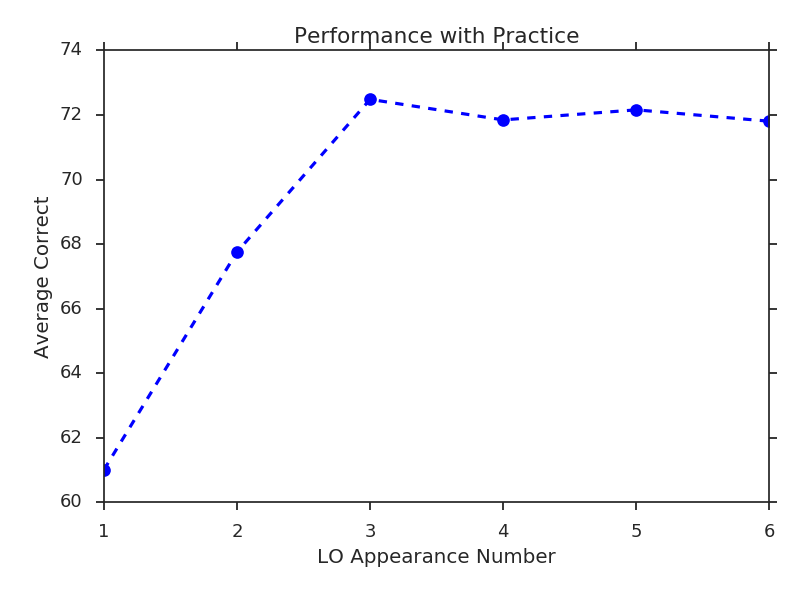
\includegraphics[height=2.75in]{perf_vs_otp}
\caption{Percent correct for all users as a function of appearance number for all LOs.}
\label{fig:Performance}
\end{figure}

There are several methods of analysis to statistically estimate the probability of improved performance at each step in the learning process.  One of the most widely used of these is Bayesian Knowledge Tracing, which was developed in the mid 1990s \cite{CorbettAnderson1995}.  Another commonly used method for measuring the growth of knowledge as study progresses is Performance Factor Analysis and its variations \cite{Pavlik2009}.  Studies are currently in progress to apply both of these methods to the data being produced by StudyWise.

\subsection{Confidence and meta-cognition}
One of the specifications for StudyWise which was agreed upon early in the development process was the desire to record not just the users' answers but to also ask the users to estimate their level of confidence in the answers they chose.  This falls into the area of learning science called metacognition, the subject of which is a learner's self-awareness of their own level of knowledge.  There is growing interest in studying the relationship between a learner's self-confidence and self-knowledge and their overall learning performance \cite{Aghababyan2017}.

\section{Data Visualization}

A very important part of the exploration and analysis of large data sets in education is the use of visualization.  In the environment we are using for the StudyWise data, there are a range of tools available for this.  The Python and R computer languages have several powerful visualization packages available.  All of these are available from within the Databricks environment.

\subsection{Data Exploration and visualization using built-in tools}

A very common method of organizing the analysis of large data sets is through the use of computing notebooks.  In this model, computations in Python, R, Scala or SQL can be interspersed with visualizations and graphs which facilitates the exploration of the data.  This can include basic plots of daily usage of the system and extend to very sophisticated learning science and statistical analysis.

Computing languages such as Python, R and Scals have computing notebook systems available such as Jupyter \url{http://jupyter.org} (an outgrowth of the earlier iPython noteooks).  Another open source notebook, Apache Zepplin \url{http://http://zeppelin.apache.org/}, supports Apache Spark, Python and SQL.  In order to optimize the use of their computing environment, however, Databricks has developed their own proprietary notebook which can run Apache Spark code through the use of Scala, Python (Pyspark), R (RSpark) or SQL (SparkSQL).

The Databricks environment also includes a file system, called the Databricks File System (DBFS) which is a front end for Amazon S3 and which facilitates the organization of and access to very large data sets.  Through DBFS, data can be read into a notebook for analysis.  The notebooks also include built in plotting routines which allows the quick construction of histograms, scatter plots, line plots, bar charts, pie charts, pivot tables, geographic maps, and others.

In addition to the quick, built-in plotting methods, the notebooks also have available the very powerful plotting routines built into Python, such as Matplotlib, Seaborne, and Bokeh and ggplot2 in R and Python.  Thus the exploration, analysis, and visualization of large data set can be done within the context of a Databricks notebook.   This facilitates the organization of the research as well as making it very easy to share results and to collaborate on research without having to duplicate code.  There is also an interface to Github \url{https://github.com/} to allow detailed tracking and versioning of software.
  
\section{Relationship Between Research and Production}

Much of the research done on large educational data sets is done with the goal of making improvements to existing products.  Such research can result in updates to the data API, adaptive algorithm, or educational design of a product.  Product targeted research projects may result in analyses which can directly provide feedback to users to help improve their educational outcomes.

In other cases, the outcome of the research could be a contribution to fundamental learning science which might not be immediately incorporated into the product from which the data was produced but will inform future development of other educational products.

The computing environment used for StudyWise allows for all of these possibilities.  Cloud computing, such as AWS and Databricks, allows separate computing clusters to be set up for each project.  Cloud storage, such as S3, can also be managed to direct data streams for a particular purpose and to also set up secure, isolated storage locations so that access can be carefully controlled.  This allows projects that must use PII data, for example, to be clearly distinct from those that do not.

\subsection{Development, Test and Production Environment}

StudyWise is a commercially available software product and has been developed in a way consistent with its commercial nature.

In particular, each of the components of the data transmission and processing pipeline have separate development, test, and production versions.  This includes data intake, verification, and storage, with separate servers and S3 storage for each function.  There are also unique data streams and processing computing clusters for each stage of development

This allowed the developers to send trial data messages to a development area while the Analytics API was being developed and refined.  These messages would vary in format while the API was being finalized and refined.  

During acceptance testing, a separate test area would have only data messages which, ideally, conform to the final format but which were not produced by actual users.  This area can also be used to test the scalability of the application without interfering with end users.

The production area is reserved for actual user data from the end users.  It is also the area which will need to be able to scale up as usage expands, although this functionality can be prototyped in the test environment.

This separation of environments allows modifications to be made to the software, the analytics data API, and the overall infrastructure without interfering with use by the real users.  The fact that all of these components were built upon cloud-based serviced means that each could be implemented and tested without the need to acquire dedicated hardware for either storage or computing.

\subsection{Software Development Life Cycle for Educational Apps}

Up until recently, the research upon which an educational application was based would have been done on systems quite different from those upon which the production version would run.  In particular, research groups often used computer languages, such as Matlab, which work well for doing research but are not designed to scale up for production systems.

A great advantage of using a framework like Apache Spark is that it can be used by data scientists and learning scientists to design and produce new algorithms and new processing streams which can then be moved in to a production system with far less modification than was often the case previously.  

Spark supports the use of Scale/Java, Python, R and SQL on data from a common source and in a common format.  So if researchers find that their research requires a particular data format, the production system can, if desired, adapt this. In the case of StudyWise, for example, the use of JSON was required by the data engineering group for company-wide compatibility, but the specifics of the API were developed jointly between learning scientists, business analysts, and data engineers.

Similarly, if the data engineers working on production systems find better ways of handling large amounts of data, their experience can be leveraged by researchers for their work because they are working within the same framework and using the same set of tools.  The adoption of the Parquet file system to speed learning science analysis is an excellent example of this.  Software engineers also have tools such as those for carefully tracking the version of software, that can be very useful for keeping track of research.  

With software engineers, data engineers, data scientists, and learning scientists all working in the same computing environment, the transfer of work from research to development to testing to production is greatly facilitated.  Experience and expertise can also be shared in a way that has not been possible until the development of systems such as Apache Spark and Databricks.  Each group can have their own separate areas and separate environments, but the transfer of algorithms and reporting tools between groups is much easier.  And the development of shared expertise between groups  benefits everyone.
    
\section{Summary}

Mobile devices such as smart phones and tablets can host educational applications which can be used anywhere, anytime, at the user's convenience.  Such applications can be instrumented to emit data messages which can provide data on a user's learning progress.  The data transmission, storage, security, and analysis used for such applications can be very similar to that which has been developed for the Internet of Things, where smart devices produce data messages on how the device is used.  

Unlike most IOT devices, smart phones and tablets can also utilize on-device storage to allow the user-interaction data messages to be stored for later transmission if a network connection is not available at the moment it is generated.  This allows these educational apps to truly be used anywhere and anytime, including on airplanes or in very isolated areas where cellular data connections may not be available.

The infrastructure implemented for these mobile educational apps is now being used by about 5,000 users who are answering several thousand questions per day.  However, this infrastructure is designed to scale out to handle tens of millions of users answering millions of questions per day with no changes needed at any stage.  Using cloud computing this can all be done without the need to have a data center or to purchase any server or storage hardware.  One only needs a checkbook backed by a large enough bank account to pay for the cloud storage and computing charges.

Given the great flexibility this allows students, teachers, developers, data engineers, and learning scientists, we expect that StudyWise is just the first of many applications like it to come.  It puts learning directly into the hands of the users, directly along side of their social media apps, text messaging, games, email, and -- for the old fashioned -- phone calls.  

StudyWise uses recent results from learning science to help students master course material in an optimal way, all in the palm of their hand.  At the same time, these apps are producing large amounts of educational data which will allow the continued improvement of the educational experience and also provide fundamental insight into the learning process.

\subsubsection*{Acknowledgments.} StudyWise was developed by a team of  fifteen developers, project managers, and data scientists lead by Technical Product Manager James Cooper, Business Product Manager Katie Ward, and Engineering Lead Tom Titchener.  The infrastructure described was set up and is managed by the Data Engineering group lead by Matt Hogan and Matt Ashbourne and the Global Technology Services group lead by Boris Slavin.

\bibliographystyle{splncs03}

\bibliography{studywise_references}

\end{document}
